\documentclass[12pt,a4paper,oneside]{article}

\usepackage[utf8]{inputenc}
\usepackage[portuguese]{babel}
\usepackage[T1]{fontenc}
\usepackage{amsmath}
\usepackage{amsfonts}
\usepackage{amssymb}
\usepackage{graphicx}
\usepackage{xcolor}
\usepackage{multicol}
\usepackage{tikz}
\usetikzlibrary{automata,positioning}

% Definindo novas cores
\definecolor{verde}{rgb}{0.25,0.5,0.35}

\author{\\Universidade Federal de Jataí (UFJ)\\Bacharelado em Ciência da Computação \\Linguagens Formais e Autômatos \\Esdras Lins Bispo Jr.}

\date{14 de setembro de 2018}

\title{\sc \huge Mini-Teste 2}

\begin{document}

\maketitle

{\bf ORIENTAÇÕES PARA A RESOLUÇÃO}

\small
 
\begin{itemize}
	\item A avaliação é individual, sem consulta;
	\item A pontuação máxima desta avaliação é 10,0 (dez) pontos, sendo uma das 06 (seis) componentes que formarão a média final da disciplina: quatro mini-testes (MT), uma prova final (PF), exercícios-bônus (EB) e exercícios aplicados em sala de aula pelo método de Instrução pelos Colegas (IpC);
	\item A média final ($MF$) será calculada assim como se segue
	\begin{eqnarray}
		MF & = & MIN(10, S) \nonumber \\
		S & = & [(\sum_{i=1}^{4} max(MT_i, SMT_i ) + PF].0,2  + EB + IpC\nonumber
	\end{eqnarray}
	em que 
	\begin{itemize}
		\item $S$ é o somatório da pontuação de todas as avaliações, e
		\item $SMT_i$ é a substitutiva do mini-teste $i$.
	\end{itemize}
	\item O conteúdo exigido desta avaliação compreende o seguinte ponto apresentado no Plano de Ensino da disciplina: (2) Autômatos Finitos Determinísticos, e (3) Autômatos Finitos Não-determinísticos.
\end{itemize}

\begin{center}
	\fbox{\large Nome: \hspace{10cm}}
\end{center}

\newpage

\begin{enumerate}
	
	\section*{Segundo Mini-Teste}
	
	\item (5,0 pt) Seja o AFD M conforme o diagrama de estados a seguir.
	\begin{center}
		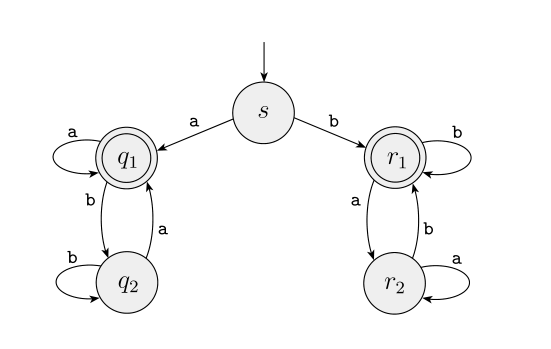
\includegraphics[width=.7\textwidth]{images/afd-m4}
	\end{center}
	Qual é a função do estado $q_2$?
	
	{\color{blue} {\bf Resposta:} A função do estado $q_2$ é registrar se a cadeia começa com {\sf a} e termina com {\sf b}, até o momento.
	}

\newpage
	
	\vspace*{2cm}
	\item (5,0 pt) Dê o diagrama de estados de AFNs com o número especificado de estados reconhecendo cada uma das linguagens a seguir. Admita em todos os itens que o alfabeto é  $\{0,1\}$.
		\begin{enumerate}
			\item {\bf [Sipser 1.7 (c)]} (2,0 pt) a linguagem \\$\{\omega$ | $\omega$ contém um número par de 0s ou contém exatamente dois 1s$\}$ com seis estados.
						
			\vspace*{0.3cm}
			
			{\color{blue}
				
				\begin{tikzpicture}[->,>=stealth,shorten >=1pt,auto,node distance=1.5cm,
				semithick]
					\node[state,initial] 	(q0)  						{$q_0$}; 
					
					\node[state, accepting]	(q1)	[above right=of q0]	{$q_1$};
					\node[state]			(q2)	[right=of q1]		{$q_2$};
					
					\node[state] 			(q3)	[below right=of q0]	{$q_3$};
					\node[state] 			(q4)	[right=of q3]		{$q_4$};
					\node[state, accepting]	(q5)	[right=of q4]		{$q_5$};
					
					\path[->] 
					
					% TRANSIÇÕES DE SÍMBOLOS a
					(q0) edge [bend left]	node {$\epsilon$} (q1)
					(q0) edge [bend right]	node {$\epsilon$} (q3)
					
					(q1) edge [bend left]	node {0} (q2)
					(q1) edge [loop above] 	node {1} ()
					
					(q2) edge [bend left]	node {0} (q1)
					(q2) edge [loop above] 	node {1} ()
					
					(q3) edge [bend left]	node {1} (q4)
					(q3) edge [loop above] 	node {0} ()
					
					(q4) edge [bend left]	node {1} (q5)
					(q4) edge [loop above] 	node {0} ()
					
					(q5) edge [loop above] 	node {0} ();
				\end{tikzpicture}
			}
		
			\item {\bf [Sipser 1.7 (e)]} (1,5 pt) A linguagem $0^*1^*0^+$ com três estados.
			
			\vspace*{0.3cm}
			
			{\color{blue}
				
				\begin{tikzpicture}[->,>=stealth,shorten >=1pt,auto,node distance=1.5cm,
				semithick]
					\node[state,initial] 	(q0)  						{$q_0$}; 
					
					\node[state]			(q1)	[right=of q0]		{$q_1$};
					\node[state, accepting]	(q2)	[right=of q1]		{$q_2$};
					
					\path[->] 
					
					% TRANSIÇÕES DE SÍMBOLOS a
					(q0) edge [bend left]	node {$\epsilon$} (q1)
					(q0) edge [loop above] 	node {0} ()
					
					(q1) edge [bend left]	node {0} (q2)
					(q1) edge [loop above] 	node {1} ()
					
					(q2) edge [loop above] 	node {0} ();
				\end{tikzpicture}
			}
		
			\item {\bf [Sipser 1.7 (g)]} (1,5 pt) A linguagem $\{ \epsilon \}$ com um estado.
			
			\vspace*{0.3cm}
			
			{\color{blue}
				
				\begin{tikzpicture}[->,>=stealth,shorten >=1pt,auto,node distance=1.5cm,
				semithick]
				\node[state,initial, accepting] 	(q0)  						{$q_0$}; 
				
				
				
				\end{tikzpicture}
			}
		\end{enumerate}

\end{enumerate}

\end{document}